%\clearpage{\pagestyle{empty}\cleardoublepage}

%\chapter{Object reconstruction}\label{chap:objects}
\section{Object reconstruction}\label{chap:objects}

After having described the ATLAS detector, in the following Section we will
explain how object (electrons, muons, jets and the missing transverse energy \met) 
are reconstructed to be used in physics analyses. In addition details from
selections common to the analyses presented in this dissertation are given.


%\section{Electrons}\label{sec:electrons}
\subsection{Electrons}\label{sec:electrons}
Electrons are reconstructed for pseudorapidities up to $|\eta| = 2.5$, where
information from the ID is available, matching a track with an energy deposit
(cluster) in the electromagnetic calorimeter. 

To identify tracks from ID points an inside-out algorithm is used, starting from a 
seed of three aligned hits in the pixel detector or in the SCT. Five fundamental parameters,
shown and described in Figure~\ref{fig:trackpar}, are computed and used for the subsequent 
steps of hits association. The candidate track must be 

\begin{figure}[tb]\begin{center}
	\subfigure[]{
  	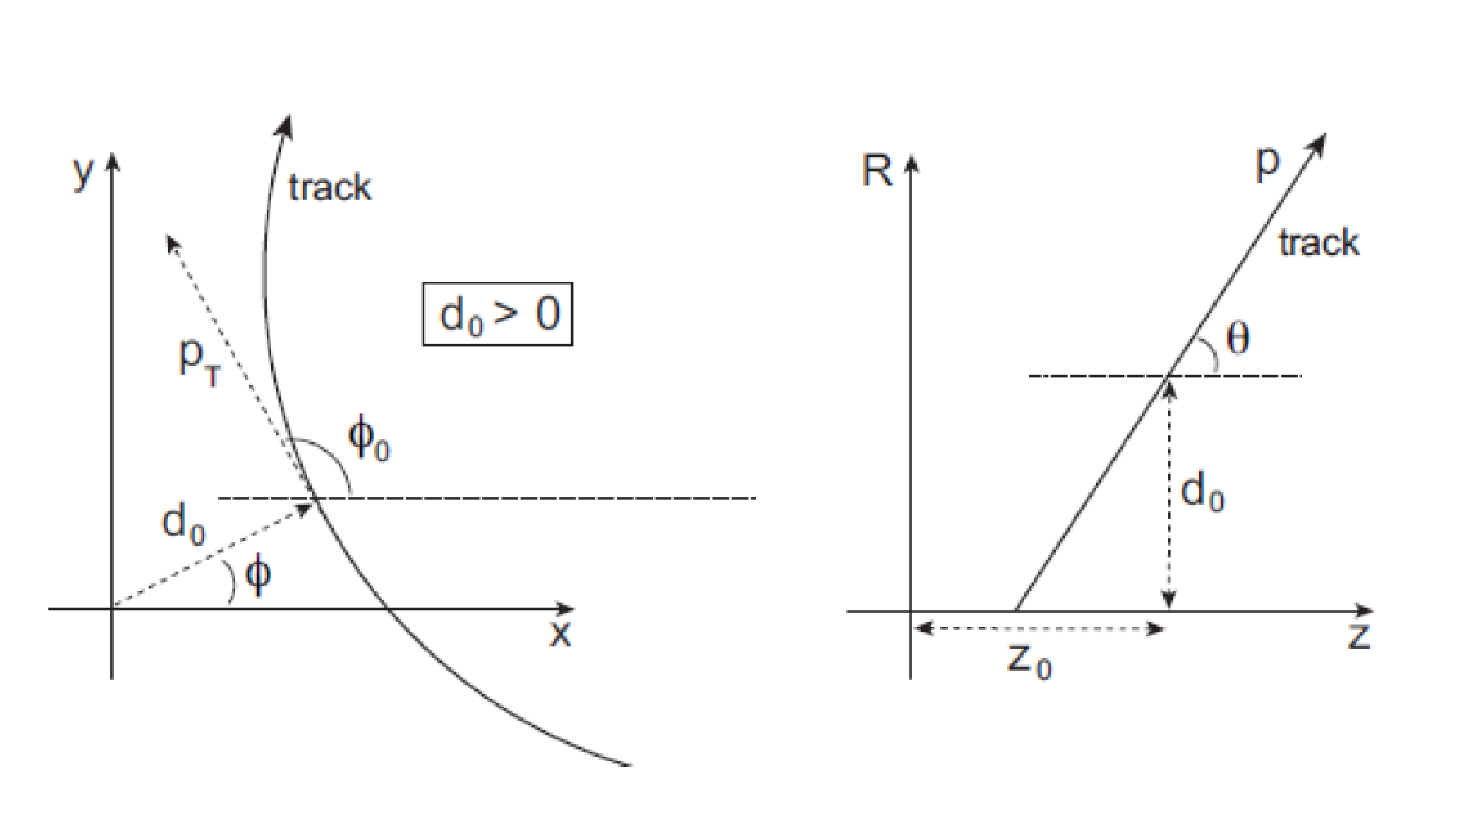
\includegraphics[width=0.7\textwidth]{objectsreconstruction/figures/tracks}}
	\caption{Schematic drawings of the parameters used for track reconstruction in the XY and $R$Z planes (left and right respectively).
          The parameters are: $q/p$, the charge divided by the momentum; $\theta$, or more used $\eta$, the angle
          with respect to the Z axis in the $R$Z plane measured from the perigee; $\phi_0$, the angle 
          with respect to the X axis in the XY plane measured from the perigee; $d_0$, the impact parameter, 
          or perigee with respect to the Z axis in the XY plane; $z_0$, Z component of the perigee.\label{fig:trackpar}}
\end{center}\end{figure}


Clusters are built starting from
$\Delta\eta\times\Delta\phi=0.025\times0.025$ single energy deposits summing
up into towers. Adjacent towers form clusters of $3\times7$ cells units in $\eta\times\phi$
in $|\eta|<1.4$ and $5\times5$ further.




excluding the transition region $1.37<|\eta| <1.52$
with inactive material.



%\section{Muons}\label{sec:muons}
\subsection{Muons}\label{sec:muons}



%\section{Jets}\label{sec:jets}
\subsection{Jets}\label{sec:jets}


%\section{Missing Transverse Energy}\label{sec:met}
\subsection{Missing Transverse Energy}\label{sec:met}
